% !TEX TS-program = pdflatex
% !TEX encoding = UTF-8 Unicode

\documentclass[11pt]{article} % use larger type; default would be 10pt

\usepackage{pgf}
\usepackage{tikz}
\usetikzlibrary{arrows,automata,shapes}
\usetikzlibrary{decorations.pathmorphing} % LATEX and plain TEX when using Tik Z

\usepackage[utf8]{inputenc} % set input encoding (not needed with XeLaTeX)

%%% PAGE DIMENSIONS
\usepackage{geometry} % to change the page dimensions
\geometry{a4paper} % or letterpaper (US) or a5paper or....
\geometry{margin=2cm} % for example, change the margins to 2 inches all round
% \geometry{landscape} % set up the page for landscape
%   read geometry.pdf for detailed page layout information

\usepackage{graphicx} % support the \includegraphics command and options
\usepackage{subcaption} % for subfigures

\usepackage{scrextend} % https://tex.stackexchange.com/questions/588/how-can-i-change-the-margins-for-only-part-of-the-text
\usepackage{color}
\definecolor{rowcolor}{rgb}{0.94, 0.97, 1.0}  % 1=weiß, 0=schwarz

% \usepackage[parfill]{parskip} % Activate to begin paragraphs with an empty line rather than an indent

%%% PACKAGES
\usepackage{booktabs} % for much better looking tables
\usepackage{array} % for better arrays (eg matrices) in maths
\usepackage{paralist} % very flexible & customisable lists (eg. enumerate/itemize, etc.)
\usepackage{verbatim} % adds environment for commenting out blocks of text & for better verbatim
%\usepackage{subfig} % make it possible to include more than one captioned figure/table in a single float
% These packages are all incorporated in the memoir class to one degree or another...
\usepackage{listings} % Absatz als Code formatieren
\usepackage{floatflt} % für floatingfigure

%%% HEADERS & FOOTERS
\usepackage{fancyhdr} % This should be set AFTER setting up the page geometry
\pagestyle{fancy} % options: empty , plain , fancy
\renewcommand{\headrulewidth}{0pt} % customise the layout...
\lhead{ZIMFLI QCoDeS Driver}\chead{}\rhead{\today}
\lfoot{Michael Wagener}\cfoot{\thepage}\rfoot{FZJ/ZEA-2}

%%% SECTION TITLE APPEARANCE
\usepackage{sectsty}
\allsectionsfont{\sffamily\mdseries\upshape} % (See the fntguide.pdf for font help)
% (This matches ConTeXt defaults)

%%% ToC (table of contents) APPEARANCE
\usepackage[nottoc,notlof,notlot]{tocbibind} % Put the bibliography in the ToC
\usepackage[titles,subfigure]{tocloft} % Alter the style of the Table of Contents
\renewcommand{\cftsecfont}{\rmfamily\mdseries\upshape}
\renewcommand{\cftsecpagefont}{\rmfamily\mdseries\upshape} % No bold!

\usepackage{longtable} % Tabellen über mehrere Seiten
\usepackage{multirow} % multirow/multicolumn
\usepackage{colortbl} % farbige Tabellenzellen
\setlength{\LTpre}{0pt}  % Remove whitespace befor and after longtables
\setlength{\LTpost}{0pt}

\setlength{\tabcolsep}{1mm} % Setzt den Längenwert von {Abstand zwischen den Spalten einer Tabelle} auf den Wert 1mm
\setcounter{tocdepth}{2}  % Tiefe des Inhaltsverzeichnisses

\setlength{\parindent}{0em} % Damit die neuen Absätze nicht eingerückt werden

%%% END Article customizations

%%% The "real" document content comes below...

\title{QCoDeS driver for the Zurich Instruments Lock-In Amplifier (ZIMFLI)}
\author{Michael Wagener}

\begin{document}
\maketitle

\tableofcontents % toc anzeigen

\ \\
%\ \\

\begin{longtable}{|p{2.7cm}|p{2.6cm}|p{10.3cm}|}
\caption{Document revision history} \\
\hline\rowcolor{rowcolor}{\bf Date} & {\bf Author} & {\bf Short description} \\
\endfirsthead
\hline
08. Mar. 2019 & M.Wagener & First edit phase. \\ \hline
 &  &  \\ \hline
\end{longtable}


\clearpage

%%%
\section{Informations}

The Zurich Instruments Lock-In Amplifier (later only ZIMFLI) will be used in the QCoDeS Framework. Therefore a driver within this framework is needed.
My work was to implement / extend the first driver version and to test it and write a user documentation (this file). \\[0.5em]
%
All tests are done with the ZIMFLI with the serial number 4039 in the ZEA-2. This device has the F5M option installed (means 5MHz insteand of 500kHz frequency range). This device was registered in our LAN during my tests. \\[0.5em]
%
I use the Spyder environment with Python 3.6.

\subsection{Git and directories}

This driver is inside the QCoDeS framework tree under {\bf Qcodes/qcodes/instrument\_drivers/ZI}. In the subdirectory {\bf TestScripts} are my scripts with all my tests. They will be described later in this document. In the subdirectory {\bf Documentation} this documentation is located. The base of the QCoDeS framework I use during my tests is the git branch \\
\centerline{\it https://github.com/qutech/Qcodes/tree/feature/qctoolkit-integration}
This driver is pushed to the git branch \\
\centerline{\it https://github.com/qutech/Qcodes/tree/feature/ziMFLI\_driver}


\subsection{Additional installations needed}

\begin{floatingfigure}[r]{0.42\textwidth}
\mbox{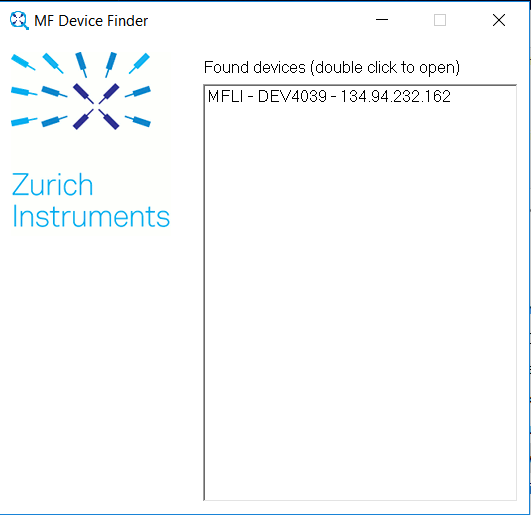
\includegraphics[width=0.4\textwidth]{ZI-DeviceFinder.png}}
\caption{ZI Device Finder}
\end{floatingfigure}
Don't forget to install the base driver from Zurich Instruments {\it https://www.zhinst.com/downloads}. Select the instrument {\it ``MFLI, MFIA''} and then the Software release version. Normally it is the best to leave the current version (for me it was 18.12). My first tests are done with the version 18.05 because the instrument has this version in its firmware. But the device runs also with the library-version 18.12. \\
Download and install the {\it Device Finder} for your Windows version or install the full packet {\it LabOne} for Windows or Linux. If you install the full packet, the documentation from ZI will also be installed.

You can connect the device to your USB port, the ZI software can install a special network driver for USB ports. After you connect the device to your network (or to your USB port), start the Device Finder and note the found device id.

Be sure that your computer is in the same subnet as the device. The device finder and later the driver cannot find the device if you use a VPN connection.

Then you have to install the Python package. From version 18.12 onwards you can start a shell and use the command
\begin{lstlisting}[frame=single]
pip install zhinst
\end{lstlisting}
All versions before have a separate download file on the ZI download page.

\clearpage


%%%
\section{General usage}

To use this driver, you have to import it and open the device. Be sure that you have the correct device id, it contains the serial number found with the {\it Device Finder}:

\begin{lstlisting}[frame=single, language=Python]
from qcodes.instrument_drivers.ZI.ZIMFLI import ZIMFLI
zidev = ZIMFLI( name='ZIMFLI', device_ID='DEV4039' )
\end{lstlisting}

During this open, the software searches for the device in the same subnet (or the USB). This will not work via VPN. The output in my test environment is:
\begin{lstlisting}[frame=single, language=Python]
Discovered device `dev4039`: MFLI with options F5M.
Creating an API session for device `dev4039` on `134.94.232.162`, `8004`
 with apilevel `6`.
\end{lstlisting}

In all following examples the variable {\bf zidev} is used as a reference to the device instance.

\ \\

After this you can access the device as decribed in detail later. As a first test you can get all version informations:
\begin{lstlisting}[frame=single, language=Python]
> import json
> print( json.dumps( zidev.version(), indent=4) )
{
    "DevType": "MFLI",
    "Options": "F5M",
    "Serial": "4039",
    "DevTime": "02.01.1970 10:41:25.265187",
    "Owner": "",
    "FPGARev": 52856,
    "DevFWRev": 53700,
    "BoardRev1": "1.4.G",
    "Copyright": "(c) 2008-2018 Zurich Instruments AG",
    "Dataserver": "ziDataServer",
    "ZI_FWRev": 0,
    "ZIRevision": 54618,
    "Version": "18.05"
}
\end{lstlisting}


\clearpage

%%%
\section{Base parameters}

The following parameter is accessible directly from the main device instance.

\begin{itemize}
\item zidev.{\bf oscillator1\_freq}( {\it value} ) \\
	Reads (without a value) or writes the frequency of the oscillator. Before writing, the driver checks the valid range from 0 Hz to 500 kHz ( or 5 MHz if the F5M option is installed).
\item zidev.oscillator2\_freq( {\it value} ) \\
	Same for the second oscillator if the MD option is installed.
\item zidev.oscillator3\_freq( {\it value} ) \\
	Same for the third oscillator if the MD option is installed.
\item zidev.oscillator4\_freq( {\it value} ) \\
	Same for the fourth oscillator if the MD option is installed.

\item zidev.{\bf bufferedReader}( demod\_index, total\_time, dolog=False, copyFreq=False, copyPhase=False, copyDIO=False, copyTrigger=False, copyAuxin=False ) \\
	Read the sample informations from the given demodulator for a given time and returns it as a dict of arrays. The parameters are:
	\begin{itemize}
	\itemsep0pt
	\item demod\_index = index of demodulator channel (1,2)
	\item total\_time  = number of seconds for measurement, this time the function is blocking
	\item dolog = Flag if this function print some informations during running (elapsed time and data length)
	\item copyFreq = Flag to copy the frequency data
	\item copyPhase = Flag to copy the phase data
	\item copyDIO = Flag to copy the digital I/O data
	\item copyTrigger = Flag to copy the trigger data
	\item copyAuxin = Flag to copy both auxin port data \\
	{\it The copy flags can be set to False (default if omitted) to preserve memory usage. Set them to True to get more arrays in the resulting dict.}
	\end{itemize}
	\textbf{\textit{Return:}} a dict with dict\_keys(['timestamp', 'x', 'y', {\it 'frequency'}, {\it 'phase'}, {\it 'dio'}, {\it 'trigger'}, {\it 'auxin0'}, {\it 'auxin1'}, 'time', 'R', 'phi'])
	The fields `R' and `phi' are calculated from `x' and `y'. The italic fields can be switched off with the copy flags. The field 'time' has the values:
	\begin{itemize}[ ]
	\itemsep0pt
	\item 'trigger': 0
	\item 'dataloss': False,
	\item 'blockloss': False,
	\item 'ratechange': False,
	\item 'invalidtimestamp': False,
	\item 'mindelta': 0,
	\item 'clockbase': 60000000.0  {\it this is used to calculate the correct time from the timestamps}
  	\end{itemize}
  	
  \item zidev.{\bf version}() \\
  	Read all possible version informations and returns them as a dict. See the first example above.

  \item zidev.{\bf Scope} \\
  	Submodule for the scope functionality. This is under development.
  	
\end{itemize}


%%%
\section{Submodules}

In this section I describe all implemented submodules for this device. For each submodule all available parameters are described.

\subsection{Demodulator}
	Combines all parameters of the parent concerning the demodulators. Parameters:
	\begin{itemize}
	\item bypass: Allows to bypass the demodulator low-pass filter, thus increasing the bandwidth.
	\item frequency: Indicates the frequency used for demodulation and for output generation. The demodulation frequency is calculated with oscillator frequency times the harmonic factor. When the MOD option is used linear combinations of oscillator frequencies including the harmonic factors define the demodulation frequencies.
	\item order: Selects the filter roll off between 6 dB/oct and 48 dB/oct. Allowed Values:
	\begin{itemize}
	\itemsep0pt
	\item 1 1st order filter 6 dB/oct
	\item 2 2nd order filter 12 dB/oct
	\item 3 3rd order filter 18 dB/oct
	\item 4 4th order filter 24 dB/oct
	\item 5 5th order filter 30 dB/oct
	\item 6 6th order filter 36 dB/oct
	\item 7 7th order filter 42 dB/oct
	\item 8 8th order filter 48 dB/oct
	\end{itemize}
	\item harmonic: Multiplies the demodulator's reference frequency by an integer factor. If the demodulator is used as a phase detector in external reference mode (PLL), the effect is that the internal oscillator locks to the external frequency divided by the integer factor.
	\item oscselect: Connects the demodulator with the supplied oscillator. Number of available oscillators depends on the installed options. Is a number between 0 and the number of oscillators -1
	\item phaseadjust: Adjust the demodulator phase automatically in order to read 0 degrees.
	\item phaseshift: Phase shift applied to the reference input of the demodulator. %Value is clipped to -180 .. +180°
	\item timeconstant: Sets the integration time constant or in other words, the cutoff frequency of the demodulator low pass filter.
	\item samplerate(*): Defines the demodulator sampling rate, the number of samples that are sent to the host computer per second. A rate of about 7-10 higher as compared to the filter bandwidth usually provides sufficient aliasing suppression. This is also the rate of data received by LabOne Data Server and saved to the computer hard disk. This setting has no impact on the sample rate on the auxiliary outputs connectors. Note: the value inserted by the user may be approximated to the nearest value supported by the instrument.
	\item sample(*): Contains streamed demodulator samples with sample interval defined by the demodulator data rate.
	\item sinc: Enables the sinc filter. When the filter bandwidth is comparable to or larger than the demodulation frequency, the demodulator output may contain frequency components at the frequency of demodulation and its higher harmonics. The sinc is an additional filter that attenuates these unwanted components in the demodulator output.
	\item signalinput: Selects the input signal for the demodulator. Possible values: 'Sig In 1', 'Curr In 1', 'Trigger 1', 'Trigger 2', 'Aux Out 1', 'Aux Out 2', 'Aux Out 3', 'Aux Out 4', 'Aux In 1', 'Aux In 2', 'Constant input'
	\item streaming(*): Enables the data acquisition for the corresponding demodulator.
	\item trigger(*): Selects the acquisition mode (i.e. triggering) or the demodulator.
        %dmtrigs = {'Continuous': 0,            #demodulator data is continuously streamed 
         %                                      #to the host computer.
          %         'Trigger in 1 Rise': 1,     #rising edge triggered.
           %        'Trigger in 1 Fall': 2,     #falling edge triggered.
          %         'Trigger in 1 Both': 3,     #triggering on both rising and falling edge.
          %         'Trigger in 2 Rise': 4,     #rising edge triggered.
          %         'Trigger in 1|2 Rise': 5,   #rising edge triggered on either input.
          %         'Trigger in 2 Fall': 8,     #falling edge triggered.
          %         'Trigger in 1|2 Fall': 10,  #falling edge triggered on either input.
          %         'Trigger in 2 Both': 12,    #triggering on both rising and falling edge.
          %         'Trigger in 1|2 Both': 15,  #triggering on both rising and falling 
          %                                     #edge or either trigger input.
          %         'Trigger in 1 Low': 16,     #demodulator data is streamed to the host
          %                                     #computer when the level is low (TTL).
          %         'Trigger in 1 High': 32,    #demodulator data is streamed to the host
          %                                     #computer when the level is high (TTL).
          %         'Trigger in 2 Low': 64,     #demodulator data is streamed to the host
          %                                     #computer when the level is low (TTL).
          %         'Trigger in 1|2 Low': 80,   #demodulator data is streamed to the host 
          %                                     #computer when either level is low (TTL).
          %         'Trigger in 2 High': 128,   #demodulator data is streamed to the host
          %                                     #computer when the level is high (TTL).
          %         'Trigger in 1|2 High': 160, #demodulator data is streamed to the host
          %                                     #computer when either level is high (TTL).

	\item x: get sample of x coordinate
	\item y: get sample of y coordinate
	\item R: get sample of absolute value of x+y*i
	\item phi: get sample of angle of x+y*i
	\item cfgTimeout: stores the  used timeout in seconds for the readings of sample data (default 0.07)
	\item (*) all parameters marked with this are only accessible for channel 1 or if the MD option is installed
	\end{itemize}


\subsection{Signal Input (Voltage)}
    Combines all the Parameters from the parent concerning the signal input. Parameters:
    
            autorange: Automatic adjustment of the Range to about two times the maximum 
                signal input amplitude measured over about 100 ms.
            range: Defines the gain of the analog input amplifier. The range should 
                exceed the incoming signal by roughly a factor two including a 
                potential DC offset. The instrument selects the next higher available
                range relative to a value inserted by the user. A suitable choice of
                this setting optimizes the accuracy and signal-to-noise ratio by 
                ensuring that the full dynamic range of the input ADC is used.
            float: Switches the input between floating (ON) and connected to ground (OFF). 
                This setting applies both to the voltage and the current input. It
                is recommended to discharge the test device before connecting or to
                enable this setting only after the signal source has been connected
                to the Signal Input in grounded mode.
            scaling: Applies the given scaling factor to the input signal.
            ac: Defines the input coupling for the Signal Inputs. 
                AC coupling inserts a high-pass filter. OFF means DC ccoupling
            impedance: Switches between 50 Ohm (ON) and 10 M Ohm (OFF).
            diff: Switches between single ended (OFF) and differential (ON) measurements.
            max: Indicates the maximum measured value at the input.
            min: Indicates the minimum measured value at the input.
            on: Enables the signal input.
            trigger: Switches to the next appropriate input range such that the range 
                fits best with the measured input signal amplitude.


\subsection{Signal Input (Current)}
    Combines all the Parameters from the parent concerning the current input
    Parameters: 
            autorange: Automatic adjustment of the Range to about two times the maximum 
                signal input amplitude measured over about 100 ms.
            range: Defines the gain of the analog input amplifier. The range should 
                exceed the incoming signal by roughly a factor two including a 
                potential DC offset. The instrument selects the next higher available
                range relative to a value inserted by the user. A suitable choice of
                this setting optimizes the accuracy and signal-to-noise ratio by 
                ensuring that the full dynamic range of the input ADC is used.
            float: Switches the input between floating (ON) and connected to ground (OFF). 
                This setting applies both to the voltage and the current input. It
                is recommended to discharge the test device before connecting or to
                enable this setting only after the signal source has been connected
                to the Signal Input in grounded mode.
            scaling: Applies the given scaling factor to the input signal.
            max: Indicates the maximum measured value at the input.
            min: Indicates the minimum measured value at the input.
            on: Enables the signal input.
            trigger: Switches to the next appropriate input range such that the range 
                fits best with the measured input signal amplitude.


\subsection{Auxilliary Inputs}
    Combines all parameters of the instrument concerning AUXInput
    Parameters:
            averaging: Defines the number of samples on the input to average as 
                a power of two. Possible values are in the range [0, 16]. A value 
                of 0 corresponds to the sampling rate of the auxiliary input's ADC.
            sample: Voltage measured at the Auxiliary Input after averaging. 
                The data rate depends on the averaging value. Note, if the instrument
                has demodulator functionality, the auxiliary input values are
                available as fields in a demodulator sample and are aligned by 
                timestamp with the demodulator output.
sample  |  Auxiliary Input sample :  {'timestamp': array([2364820144667], dtype=uint64), 'x': array([2.07443144e-07]), 'y': array([5.94475209e-07]), 'frequency': array([99999.99999991]), 'phase': array([2.2394202]), 'dio': array([0], dtype=uint32), 'trigger': array([768], dtype=uint32), 'auxin0': array([0.00133604]), 'auxin1': array([-0.00033299]), 'R': array([6.29629599e-07]), 'phi': array([70.7634789])} V


\subsection{External reference}
    Combines all the Parameters from the parent concerning the external reference
    Parameters:
            signalin: Indicates the input signal selection for the selected
                demodulator.
                Allowed Values:
                    0 = Signal Input 1
                    1 = Current Input 1
                    2 = NOT USED
                    3 = Trigger 2
                    4 = Auxiliary Output 1
                    5 = Auxiliary Output 2
                    6 = Auxiliary Output 3
                    7 = Auxiliary Output 4
                    8 = Auxiliary Input 1
                    9 = Auxiliary Input 2
%        ersigins = {'Sig In 1': 0,
%                    'Curr In 1': 1,
%                    #'Trigger 1': 2, not used in manual
%                    'Trigger 2': 3,
%                    'Aux Out 1': 4,
%                    'Aux Out 2': 5,
%                    'Aux Out 3': 6,
%                    'Aux Out 4': 7,
%                    'Aux In 1': 8,
%                    'Aux In 2': 9}
            automode: This defines the type of automatic adaptation of parameters
                in the PID used for Ext Ref.
                *** ONLY AVAILABLE IF MD OPTION IS INSTALLED. ***
                Allowed Values:
                    0 = No automatic adaption (default if no MD-option installed)
                    1 = The coefficients of the PID controller are automatically set.
                    2 = The PID coefficients, the filter bandwidth and the output
                        limits are automatically set using a LOW bandwidth.
                    3 = The PID coefficients, the filter bandwidth and the output
                        limits are automatically set using a HIGH bandwidth.
                    4 = All parameters of the PID including the center frequency
                        are adapted.
            channel: Indicates the demodulator connected to the extref channel.
            enable: Enables the external reference.
                Allowed Values:
                    OFF, ON
            locked: Indicates whether the external reference is locked.
            oscselect: Indicates which oscillator is being locked to the external
                reference.


\subsection{Signal Output}
    Combines all the parameters concerning the signal output
    Parameters:
            add: The signal supplied to the Aux Input 1 is added to the signal 
                output. For differential output the added signal is a common mode 
                offset.
            autorange: If enabled, selects the most suited output range automatically.
            differential: Switch between single-ended output (OFF) and differential 
                output (ON). In differential mode the signal swing is defined between 
                Signal Output +V / -V.
            imp50: Select the load impedance between 50 Ohm(ON) and HiZ(OFF). 
                The impedance of the output is always 50 Ohm. For a load impedance
                of 50 Ohm the displayed voltage is half the output voltage to 
                reflect the voltage seen at the load.
            offset: Defines the DC voltage that is added to the dynamic part of 
                the output signal.
            on: Enabling/Disabling the Signal Output. Corresponds to the blue 
                LED indicator on the instrument front panel.
            overloaded: Indicates that the signal output is overloaded.
            range: Sets the output voltage range. Available ranges are 0.075, 0.15,
                0.75 and 1.5
            amplitude: Sets the peak amplitude that the oscillator assigned to 
                the given demodulation channel contributes to the signal output.
                Should be given as Vpk value
                TODO To the channum a certain amplitude number is given in 
                outputamps, should it stay like that?
            ampdef: the unit for the amplitude Vpk, Vrms or dBm, default is Vpk
            enable: Enables individual output signal amplitude. When the MD 
                option is used, it is possible to generate signals being the 
                linear combination of the available demodulator frequencies.
                TODO To the channum a certain amplitude number is given in 
                outputampenable, should it stay like that?


\subsection{Auxilliary Outputs}
    Combines all parameters of the instrument concerning the AUXOutput 1-4
    Parameters:
            scale: Multiplication factor to scale the signal. 
            preoffset: Add a pre-offset to the signal before scaling is applied.
            offset: Add the specified offset voltage to the signal after scaling.
            limitlower: Lower limit for the signal at the Auxiliary Output. 
                A smaller value will be clipped. Can have a value between -10 an 10 V.
            limitupper: Upper limit for the signal at the Auxiliary Output. 
                A larger value will be clipped. Can have a value between -10 an 10 V.
            channel: channel according to the selected signal source
            output: signal source of the signal to amplify 
            value: Voltage present on the Auxiliary Output.
                Auxiliary Output Value = (Signal+Preoffset)*Scale+Offset


\subsection{Trigger Inputs}
    Combines all the Parameters concerning the TriggerInput
    Parameters:
            autothreshold: Automatically adjust the trigger threshold. The level
                is adjusted to fall in the center of the applied transitions.
            level: Trigger voltage level at which the trigger input toggles between
                low and high. Use 50% amplitude for digital input and consider the
                trigger hysteresis.


\subsection{Trigger Outputs}
    Combines the parameters concerning the TriggerOutput
    Parameters: 
            pulsewidth: Defines the minimal pulse width for the case of Scope events
                written to the trigger outputs of the device.
            source: Select the signal assigned to the trigger output.
                Possible values: 'disabled', 'osc phase of demod 2'(trigger output channel 1)
                    'osc phase of demod 4'(trigger output channel 2), 
                    'Threshold Logic Unit 1', 'Threshold Logic Unit 2',
                    'Threshold Logic Unit 3', 'Threshold Logic Unit 4',
                    'MDS Sync Out'


\subsection{Digital Input / Outputs}
    Combines all the parameters concerning the digital input/output
    Parameters:
            decimation: Sets the decimation factor for DIO data streamed to the 
                host computer.
            drive: When on, the corresponding 8-bit bus is in output mode. 
                When off, it is in input mode. Bit 0 corresponds to the least 
                significant byte. For example, the value 1 drives the least significant
                byte, the value 8 drives the most significant byte.
            extclk: OFF: internally clocked with a fixed frequency of 60 MHz
                    ON:  externally clocked with a clock signal connected to DIO Pin 68.
                         The available range is from 1 Hz up to the internal clock
                         frequency
            mode: Manual: Manual setting of the DIO output value.
                  Threshold unit: Enables setting of DIO output values by the 
                      threshold unit.
            output: Sets the value of the DIO output for those bytes where 'drive'
                is enabled.


\subsection{Multi device synchronization}
    Combines all the Parameters concerning the multi device sync
    Parameters:
            armed: Indicates whether the mds module is armed and waiting
                   for pulses, ReadOnly.
            drive: Enables output of synch pulses on trigger output 1.
            enable: Enables the mds module.
            source: Select input source for mds synch signal.
            syncvalid: Indicates if sync pulses are received, ReadOnly.
            timestamp: Used to set the resulting adjusted timestamp.
NO VALIDATOR AND NOT TESTED


\subsection{Scope Channel}
        ** under development ***


\subsection{PID}
    Combines all parameters concerning the PIDs
    These Parameters are only available if the MF-PID Quad PID/PLL Controller 
    option is installed on the MFLI parent Instrument


\subsection{Sweeper}
        if "MD" in self.options:
            self.sweeper = self.daq.sweep()
            self.sweeper.set('sweep/device', self.device)

class SweeperChannel(InstrumentChannel):
    Combines all the parameters for the sweeper module.

class Sweep(MultiParameter):
    Parameter class for the ZIMFLI instrument class for the sweeper.
    The get method returns a tuple of arrays, where each array contains the
    values of a signal added to the sweep (e.g. demodulator 4 phase).


\end{document}
